\documentclass{scrartcl}
\usepackage[a4paper,left=1in,right=1in,top=1.2in,bottom=1in]{geometry}
\usepackage{siunitx}
\usepackage{graphicx}
\usepackage{mathtools}
\usepackage{amsmath}
\usepackage{amssymb}
\setkomafont{disposition}{\normalfont\bfseries}
\newcommand*\diff{\mathop{}\!\mathrm{d}}
\newcommand*\Diff[1]{\mathop{}\!\mathrm{d^#1}}
%title
\title{Exercise 03:\\Leaky Integrate \& Fire Neuron}
\subtitle{Theoretical Neuroscience I}
\author{Maria del Cerro \and Johannes G\"atjen \and Lorena Morton}

%use these for structure/overview
\newcommand\Question{%
  \textbf{Question:}%
}
\newcommand\Answer{%
  \textbf{Answer:}%
}

\begin{document}
\maketitle
\section{Simulation of a leaky integrate-and-fire neuron}

\Question\\
Plot the input current and the membrane voltage for a leaky integrate-and-fire neuron for a constant input current, an input current of low frequency and a linearly increasing input current. Use the following parameter values:

\begin{equation*}
r_m = 1.5 \si{\mega\ohm\square\milli\meter} \qquad c_m = 20 \si{\nano\farad\per\square\milli\meter} \qquad E_L= V_\mathrm{reset}= V_0 = -65 \si{mV} \qquad V_\mathrm{thresh} = -50 \si{mV}
\end{equation*}

Also compute the inter-spike-intervals.
\\

\Answer\\

\begin{itemize}
\item
Constant input current (Figure \ref{constant}): The membrane voltage rises exponentially until it reaches the threshold value of -50 \si{mV}. The neuron fires and the membrane voltage gets reset to $V_\mathrm{reset}$. As the input current does not change this is repeated over and over. The inter-spike-intervals are all equal, i.e. the spike rate is constant.
\item
Low frequency input current (Figure \ref{low}): The amplitude of the input current is not large enough for the membrane voltage to cross the threshold value to fire. As a result there are no spikes, and the membrane voltage behaves the same as for the single compartment model up to an offset of $E_L$.
\item
Ramping input current (Figure \ref{ramp}): The input current slowly increases over time. The membrane current first rises slowly, until it reaches $V_\mathrm{thresh}$ for the first time. The neuron fires and the membrane voltage is reset, then rises again, as the input current is still high enough to elicit another spike and continues to rise. After every spike the gradient of the membrane voltage is higher than after the last, because the input current is higher. Consequently the inter-spike-intervals also get shorter over time. This can also be seen in Figure \ref{intervals}, where the inter-spike-intervals are plotted against the spike number. Apparently the inter-spike-interval length decreases exponentially.
\end{itemize}


\begin{figure}
\centering
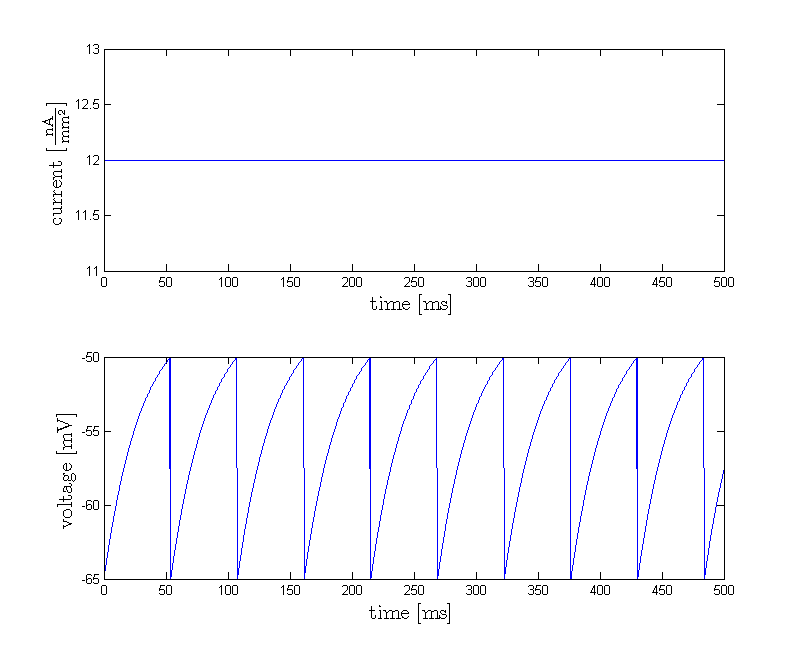
\includegraphics[trim = {1.1cm 0 1.7cm 1.1cm}, width=\textwidth, clip]{../pics/constant}
\caption{Top: The constant input current of 12 \si{\nano\ampere\per\square\milli\meter} plotted against time. Bottom: The resulting membrane voltage over time.}
\label{constant}
\end{figure}

\begin{figure}
\centering
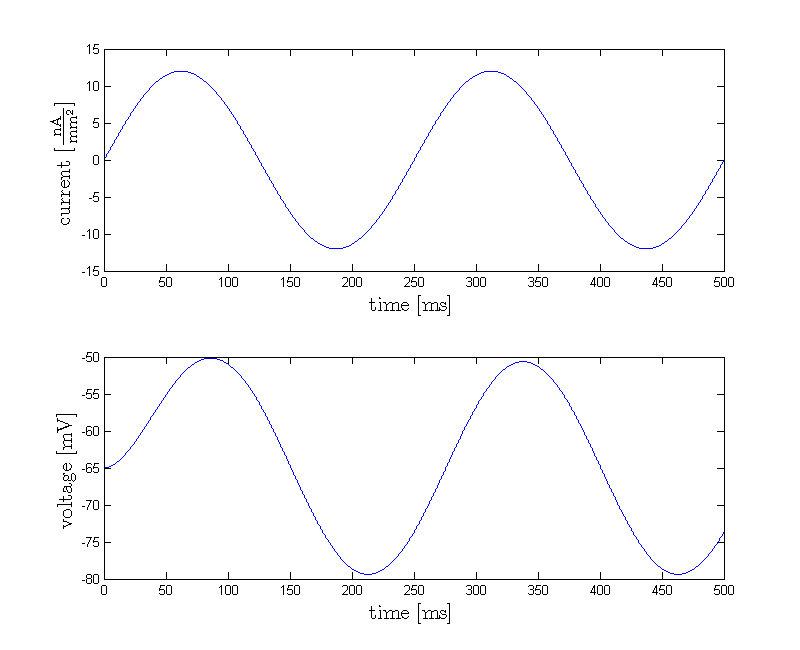
\includegraphics[trim = {1.1cm 0 1.7cm 1.1cm}, width=\textwidth, clip]{../pics/low}
\caption{Top: The low frequency (4 \si{Hz}) input current $i_e(t) = 12 \si{\nano\ampere\per\square\milli\meter} \cdot \sin{(2\pi4t)}$ plotted against time. Bottom: The resulting membrane voltage over time.}
\label{low}
\end{figure}

\begin{figure}
\centering
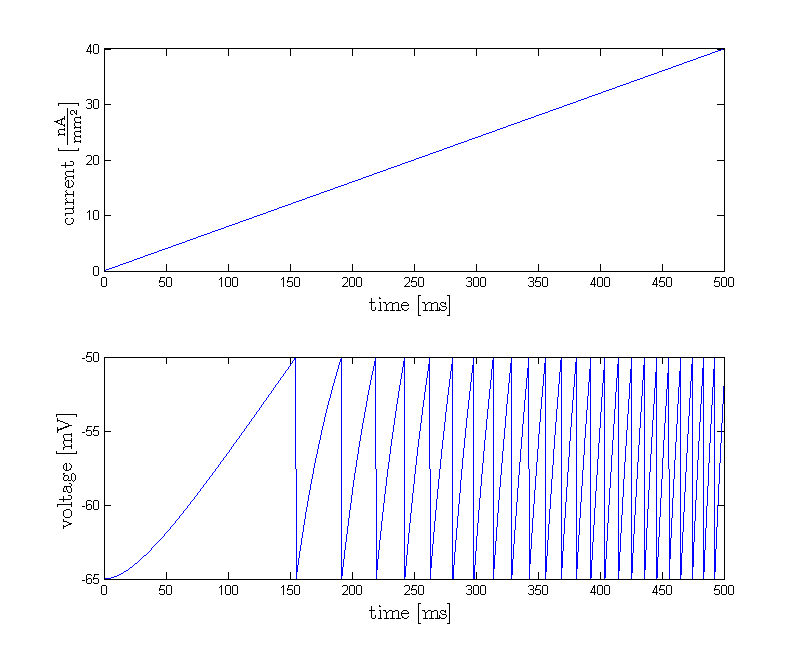
\includegraphics[trim = {1.1cm 0 1.7cm 1.1cm}, width=\textwidth, clip]{../pics/ramp}
\caption{Top: The ramping input current $i_e(t) = 12 \si{\nano\ampere\per\square\milli\meter} \cdot t / 150 \si{ms}$ plotted against time. Bottom: The resulting membrane voltage over time.}
\label{ramp}
\end{figure}

\begin{figure}
\centering
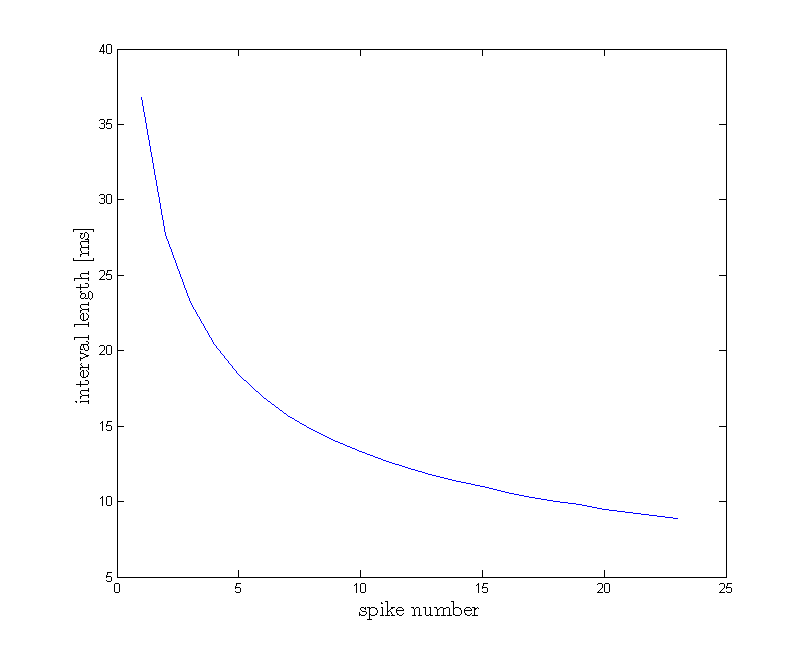
\includegraphics[trim = {1.3cm 0 1.8cm 0.9cm}, width=0.7\textwidth, clip]{../pics/ramp_intervals}
\caption{The inter-spike-interval length as a function of the number of spikes generated so far.}
\label{intervals}
\end{figure}

%lots of figures
%\begin{figure}
%\centering
%\includegraphics[trim = {1.3cm 0 2cm 0.9cm}, width=\textwidth, clip]{../pics/picname}
%\caption{caption text}
%\label{label}
%\end{figure}

\section{Optional assignment}

\Question\\
Analytically solve the dynamical equation 
\begin{equation*}
\frac{\diff V_m(t)}{\diff t} = \frac{1}{\tau_m}\left( r_m \cdot i_e(t) + E_L - V_m(t)\right)
\end{equation*}
over a time interval $\Delta t$, to derive the numerical iteration rule
\begin{equation*}
V_m(t+\Delta t) = V_m(t) \exp\left(-\frac{\Delta t}{\tau_m}\right) + \left(i_e(t) \cdot r_m + E_L \right) \left( 1 - \exp{\left( -\frac{\Delta t}{\tau_m}\right)}\right).
\end{equation*}

\Answer\\
Like in the single compartment model, the membrane potential relaxes towards an equilibrium potential as long as the membrane potential is below the threshold potential. Since we assume $i_e(t)$ to be constant over small intervals, we can say that $V_\infty = r_m \cdot i_e(t) + E_L$ and replace it in our dynamical equation and the numerical iteration rule for easier readability.

\begin{equation}
\frac{\diff V_m(t)}{\diff t} = \frac{1}{\tau_m}\left( V_\infty - V_m(t)\right)
\label{dynamic}
\end{equation}

\begin{equation*}
V_m(t+\Delta t) = V_m(t) \exp\left(-\frac{\Delta t}{\tau_m}\right) + V_\infty \left( 1 - \exp{\left( -\frac{\Delta t}{\tau_m}\right)}\right)
\end{equation*}
With some rearrangement we obtain:
\begin{equation}
V_m(t+\Delta t)= V_\infty + e^{-\frac{\Delta t}{\tau_m}}\left( V_m(t) -V_\infty\right)
\label{numeric}
\end{equation}

The solution to the dynamical equation is 
\begin{equation}
V_m(t) = V_\infty + e^{-\frac{t}{\tau_m}}(V_m(0) - V_\infty).
\label{solution}
\end{equation}


We prove this by substituting the derivation of equation \ref{solution} 
\begin{equation}
\frac{\diff V_m(t)}{\diff t} = -\frac{1}{\tau_m}(V_m(0) - V_\infty) e^{-\frac{t}{\tau_m}}
\end{equation}

in the left-hand side of equation \ref{dynamic} and equation \ref{solution} in the right-hand side of equation \ref{dynamic}.

\begin{align*}
-\frac{1}{\tau_m}(V_m(0) - V_\infty) e^{-\frac{t}{\tau_m}} &= \frac{1}{\tau_m}\left[ V_\infty - V_\infty - e^{-\frac{t}{\tau_m}}(V_m(0) - V_\infty)\right]\\
\shortintertext{The $V_\infty$'s on the right side cancel each other and we have:}
-\frac{1}{\tau_m}(V_m(0) - V_\infty) e^{-\frac{t}{\tau_m}} &= -\frac{1}{\tau_m}(V_m(0) - V_\infty) e^{-\frac{t}{\tau_m}}
\end{align*}

Since $V_m(0)$ is the membrane starting potential, in the case of $V_m(t+\Delta t)$ we can substitute $V_m(0)$ with $V_m(t)$ and $t$ with $\Delta t$ in equation \ref{solution} and arrive at equation \ref{numeric}:
\begin{equation*}
V_m(t+\Delta t) = V_\infty + e^{-\frac{\Delta t}{\tau_m}}\left( V_m(t) -V_\infty\right)
\end{equation*}
\hfill $\square$

\end{document}